\documentclass{article}
\usepackage{graphicx}
\usepackage[utf8]{inputenc}
\usepackage[fleqn]{amsmath}
\usepackage{titling}
\usepackage{graphicx,wrapfig,lipsum}
\usepackage{amssymb}
\usepackage{listings}
\usepackage[font=small,labelsep=none]{caption}
\usepackage{array}% http://ctan.org/pkg/array
\usepackage{lipsum}
\usepackage{subcaption}
\usepackage{float}
\usepackage{hyperref}


\setlength{\droptitle}{-10em}

\title{Project 4}\vspace{-3ex}
\author{Benedicte Allum Pedersen, Emil Helland Broll and Fredrik Oftedal Forr}
\date{\vspace{-5ex}}

\begin{document}

\begin{titlepage}
  \centering
  
\includegraphics[width=0.15\textwidth]{./pics/uio.png}\par\vspace{1cm}
  {\scshape\LARGE Universitetet i Oslo\par}
  \vspace{1cm}
  {\scshape\Large Project 5\par}
  \vspace{1.5cm}
  {\huge\bfseries Making a model for the solar system using ordinary differential equations\par}
  \vspace{2cm}
  {\Large\itshape Benedicte Allum Pedersen, Fredrik Oftedal Forr og Emil Helland Broll\par}
	\vfill

  \vfill
  {\large 24. november 2019\par}
\end{titlepage}

\section*{Abstract}

\tableofcontents

\newpage

\section{Introduction}
We have used the velocity Verlet algorithm for solving coupled ordinary differential equations and object orientation for making a model for the soslar system. The equations we have used for this is based on Newton's law of motion due to the gravitational force.

For a hypothetical solar system with only the Earth and the Sun Newton's law is given by one force $F_G$

\begin{flalign}
    F_G =\frac{GM_{\odot}M_{Earth}}{r^2}
\end{flalign}

In the above equation $M_{\odot}$ and $M_{Earth}$ is the mass of the Sun and the Earth. G is the gravitational constant and r is the distance between the Earth and the Sun. We neglect the motion of the Sun and only look at the motion of the Earth relative to the Sun. We can do this because we assume that the mass of the Sun is much larger than the mass of the Earth. The gravitiational force consits of a x and y component $F_{G,x}$ and $F_{Gy}$, we then use Newton's second law and obtain:

\begin{flalign}
    \frac{d^2x}{dt^2} = \frac{F_{G,x}}{M_{Earth}} \ \
    \text{and} \ \
    \frac{d^2y}{dt^2} = \frac{F_{G,y}}{M_{Earth}}
\end{flalign}

We use that the average distance bewteen the Earth and the Sun is $1.5 \cdot 10^{11}$ m and we call this one astronomical unit (1 AU). We use the masses of the different planets including the Sun that are given in \href{http://compphysics.github.io/ComputationalPhysics/doc/Projects/2019/Project5/SolarSystem/pdf/SolarSystem.pdf}{the description of Project 5}.

\section{Method}
We assume that the orbit of the Earth is circular around the Sun, we then have that:

\begin{flalign}
    F_G = \frac{M_{Earth}v^2}r = \frac{GM_{\odot}M_{Earth}}{r^2}
    \label{eq:FG}
\end{flalign}

We then solve for $v^2r$, where $v$ is the velocity of Earth.

\begin{flalign}
    v^2r = G M_{\odot} = 4\pi^2 \ \ AU^3/(yr)^2
    \label{eq:v2r}
\end{flalign}

where yr is short for years, which we use instead of seconds to decribe the motions in the solar system. We then solve this equation using Euler´s forward algorithm and the velocity Verlet method. The description of the mathematics behind this algorithm can be found in the \href{http://compphysics.github.io/ComputationalPhysics/doc/pub/ode/pdf/ode-print.pdf}{Lecture slides}.

For a system with more than one planet we need to add the magnitude of the force between Earth and the other planet, for example jupiter which is the most massive planet in the solar system. This force is given by

\begin{flalign*}
    F_{Eart-Jupiter} = \frac{GM_{Jupiter}M_{Earth}}{r^2_{Earth-Jupiter}}
\end{flalign*}

where $M_Jupiter$ is the mass of Jupiter and $r_{Earth-Jupiter}$ is the distance between Earth and Jupiter. To extend the model for all the planets in the solar system we add the other planets in the same way and choose the initial positions and velocities for all the planets from \href{https://ssd.jpl.nasa.gov/horizons.cgi#top}{NASA}.

\subsection{Object orientation}
 We make a system which contains different classes, including the planet class which is a own class in it self $\smiley$


\section{Results}
We have solved equation \ref{eq:v2r} using both Euler's forward algorithm and the velocity Verlet method. We saw that Euler's algorithm requiers a lot more calculation steps to become accurate than the Verlet algorithm. Euler's algorithm requires $5 \cdot 10^6$ steps while the Verlet algorithm requires only 500 steps. If we run our code with 100 000 integration points Euler takes 23.8 ms and uses 17 N flops while Verlet uses 35.7 ms with 38 N flops. We have therefore used the velocity Verlet method to calculate and plot the position, the energy and the angular momentum of the Earth. The results can be found in Figure \ref{fig:position}, \ref{fig:energy} and \ref{fig:am}. The plot of the energy(Figure\ref{fig:energy}) is obtained by a sum of the potential and the kinetic energy From these figures we can see that the energy and the angular momentum is conserved. These properties is consereved because if they were not conserved the Earth would not be in orbit with around the Sun.

\begin{figure}[H]
    \begin{center}
        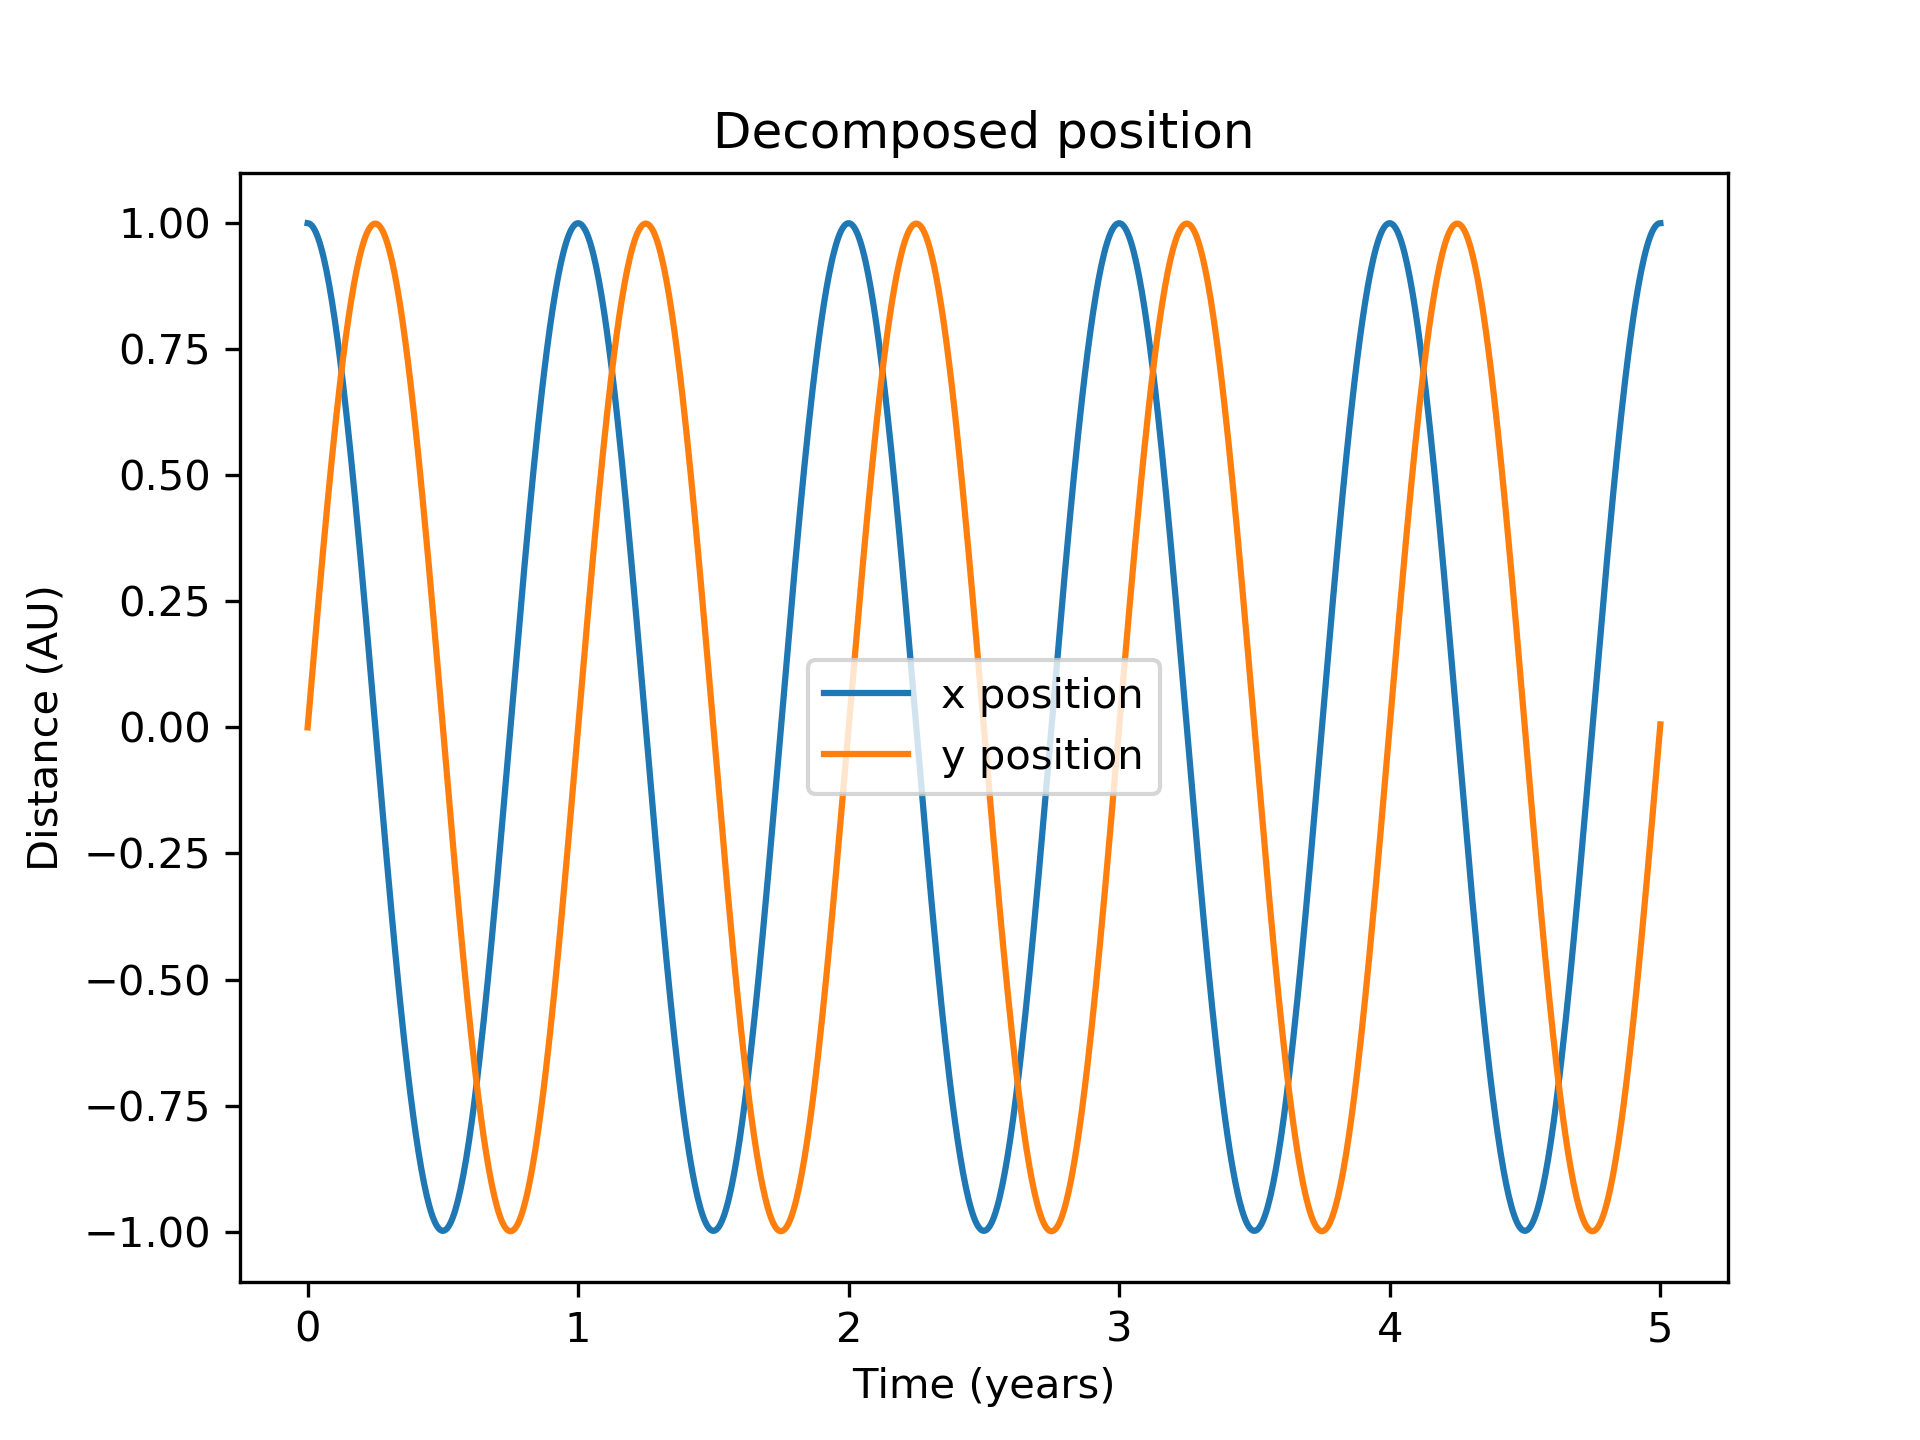
\includegraphics[width=\textwidth]{./Plot/xy_vs_time.png}
        \caption{: }
        \label{fig:position}
    \end{center}
\end{figure}

\begin{figure}[H]
    \begin{center}
        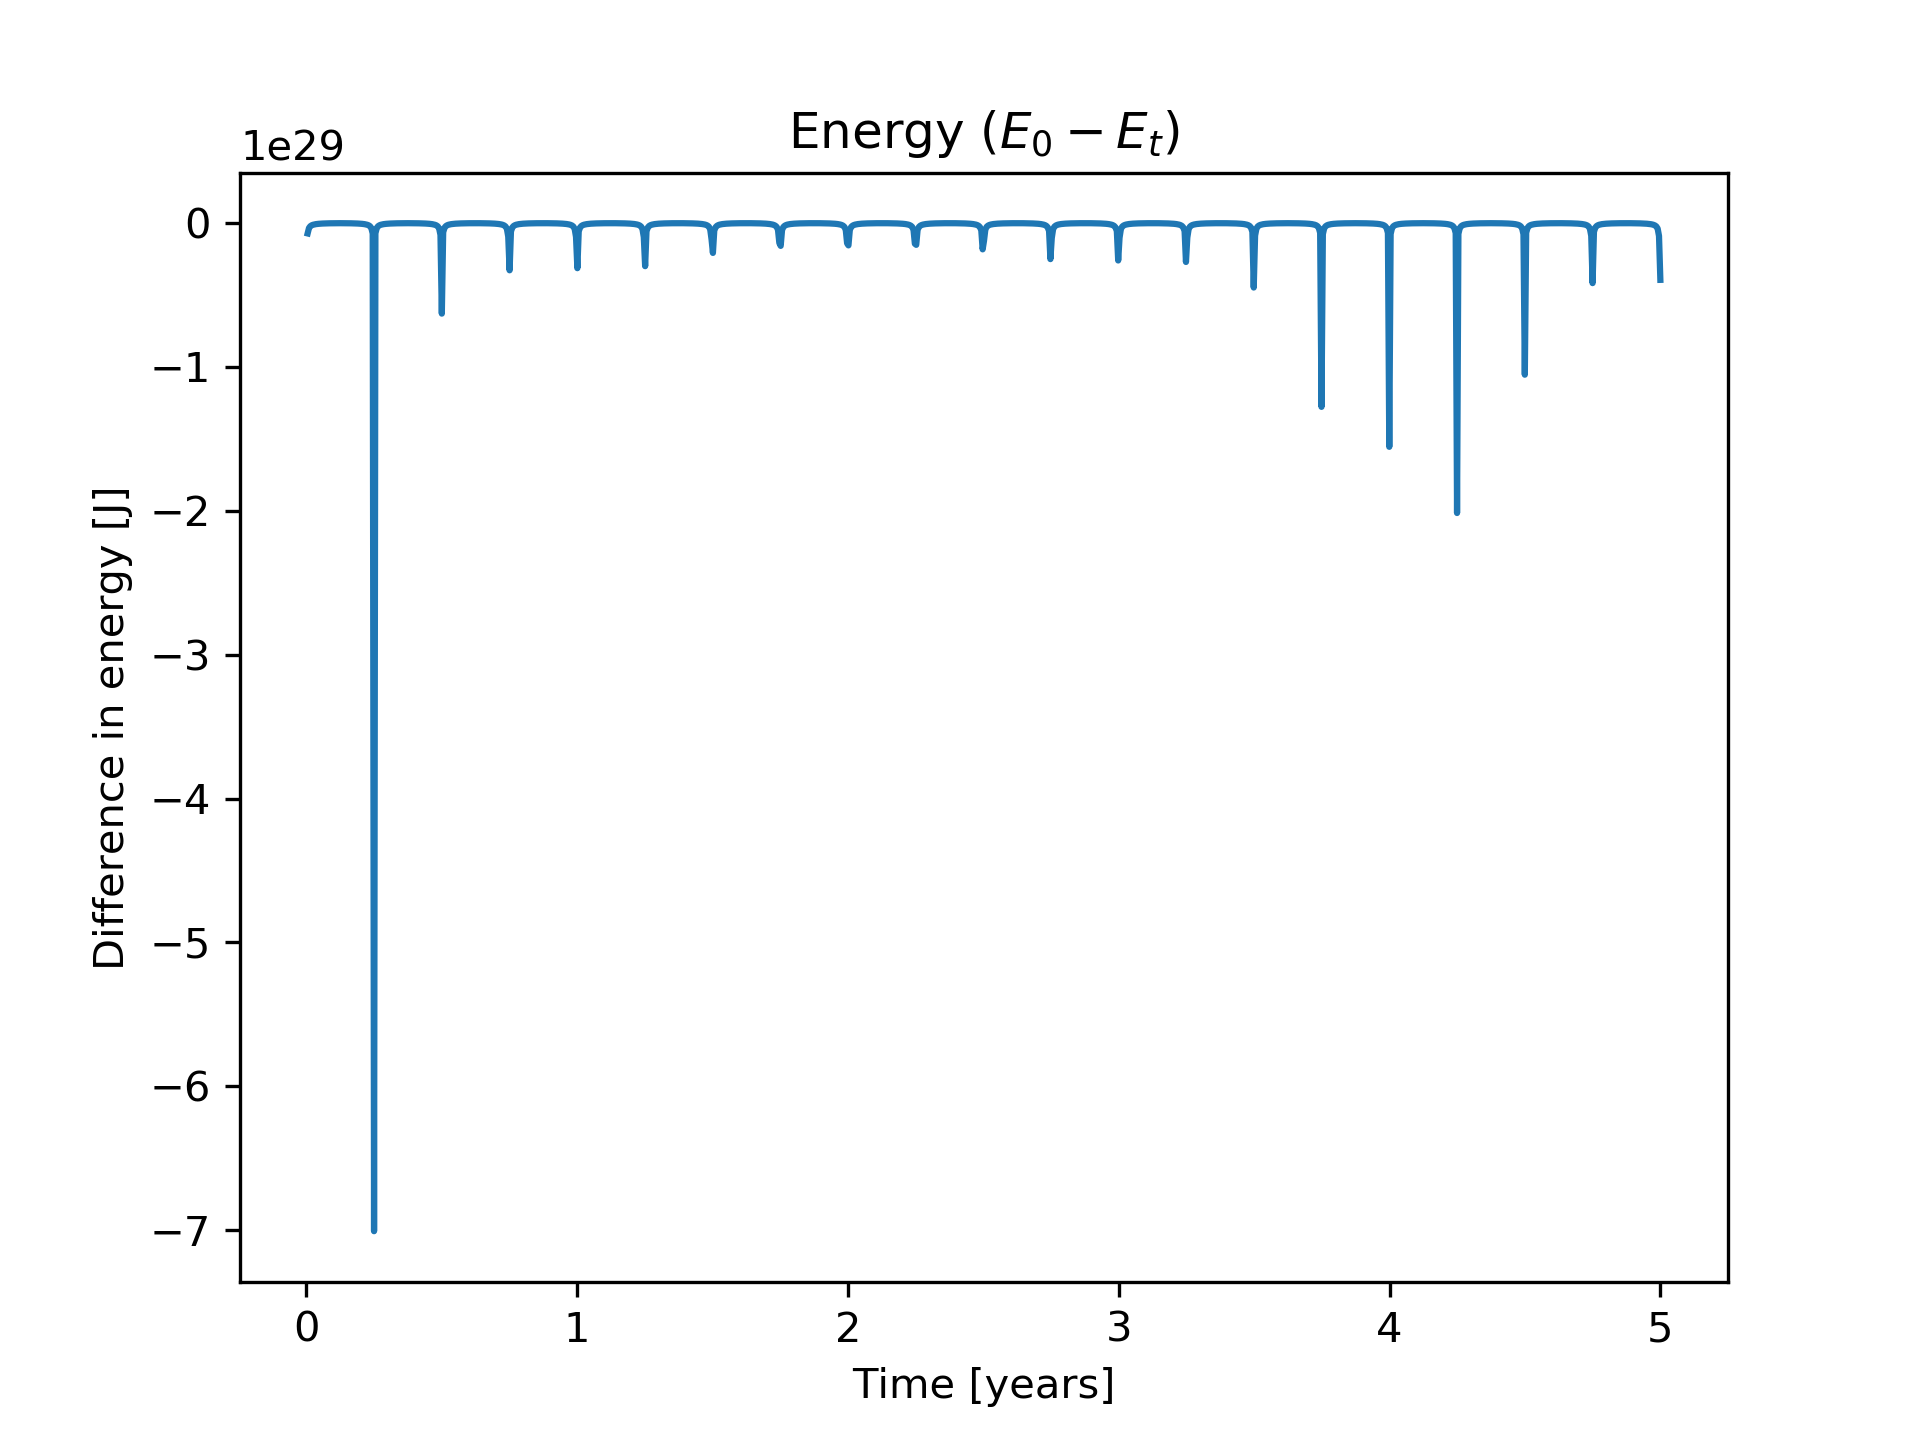
\includegraphics[width=\textwidth]{./Plot/energy.png}
        \caption{: Energy}
        \label{fig:energy}
    \end{center}
\end{figure}

\begin{figure}[H]
    \begin{center}
        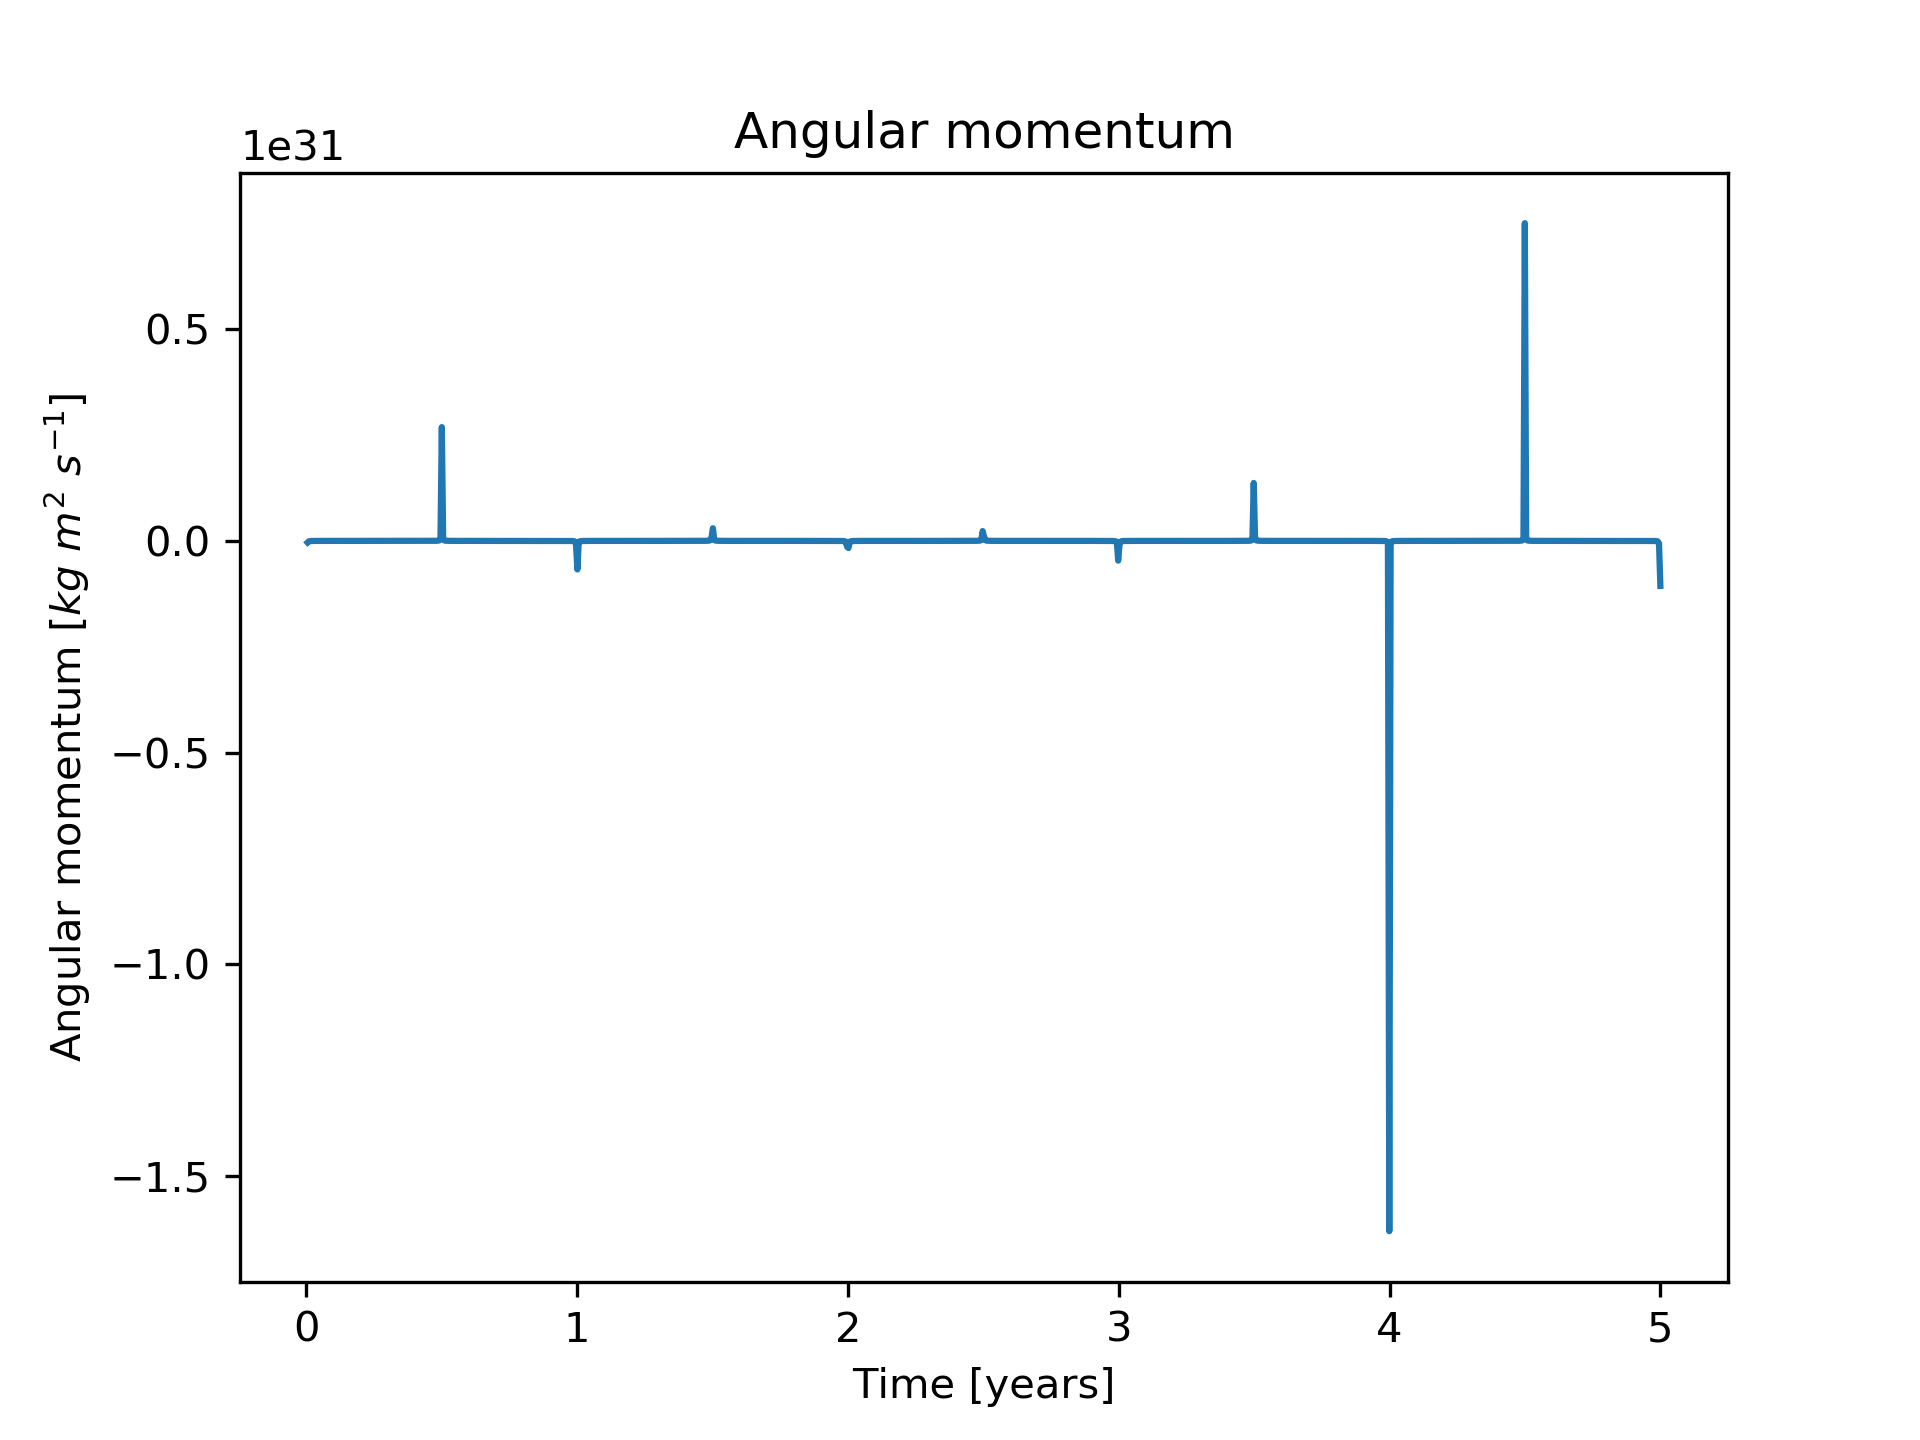
\includegraphics[width=\textwidth]{./Plot/angular_momentum.png}
        \caption{: Angular Momentum}
        \label{fig:am}
    \end{center}
\end{figure}

The initial velocity needs to be minimum 2$\pi$ AU/(yr) to obtain a circular orbit of the Earth around the Sun. We have seen this both in our code but we can also see this in the mathematics.

\begin{flalign*}
    \frac{mv^2}r &= \frac{GM_{\odot}M_E}{r^2}\\
    v^2 &= \frac{GM_{\odot}}r\\
    v &= \sqrt{\frac{4\pi^2}1} = 2\pi
\end{flalign*}

%Plot of the Eart orbiting the Sun

% Er all energi bevart kinetisk og potensiell, og angular_momentum hvorfor er de konservert?

We then consider a planet which begins at a distance 1 AU from the Sun, the inital velocity at when the planets begin to escape from the Sun is at 2.79$\pi$ AU/(yr), this means that at this inital velocity the planets orbits is no longer circular. This numerical value is quite accurate compared to the exact value. We can calculate this escape velocity exact by considering the work needed to move a planet over a small distance dr against the attractive force the planet feels. This work is given by:

\begin{flalign*}
    dW &= F_G dr = -\frac{GM_{\odot}M_E}{r^2}\\
    W &= \int_r_0^\infty - G\frac{M_{\odot}M_E}{r^2} = -G \frac{M_{\odot}M_E}{r_0}
\end{flalign*}

This gives the minimal kinetic energy to be able to reach infinity, therefore the escape velocity $v_0$ satisfies

\begin{flalign*}
    W + K &= 0 \rightarrow \frac{1}2 M_Ev_0^2 = G\frac{M_{\odot}M_}{r_0}\\
    v_0 &= \sqrt{\frac{2GM_{\odot}}r_0} = \sqrt{2\cdot4\pi^2} AU/yr = 2.8\pi AU/yr
\end{flalign*}

If we try to replace the gravitaional force from Equation \ref{eq:FG} with

\begin{flalign*}
    F_G = \frac{GM_{\odot}M_E}{r^{\beta}}
\end{flalign*}

with $\beta \in [2,3]$. When $\beta$ = 2.



\section{Discussion}

%Forskjeller mellom Verlet og Euler når vi tester algoritmene
%Time de og

\section{Appendix}

\section{Bibliography}

\begin{figure}[H]
    \begin{center}
        \includegraphics[width=\textwidth]{./Plot/}
        \caption{: }
        \label{}
    \end{center}
\end{figure}

https://en.wikipedia.org/wiki/Escape_velocity



\end{document}
